% !TEX root = ../om_ts_03.tex

\begin{frame} % название фрагмента

\videotitle{ETS: мультипликативные компоненты}

\end{frame}



\begin{frame}{ETS: мультипликативные компоненты}
  \begin{itemize}[<+->]
    \item Мультипликативные составляющие.
    \item Формулы для прогнозов.
  \end{itemize}

\end{frame}


\begin{frame}
  \frametitle{Разная амплитуда колебаний}

  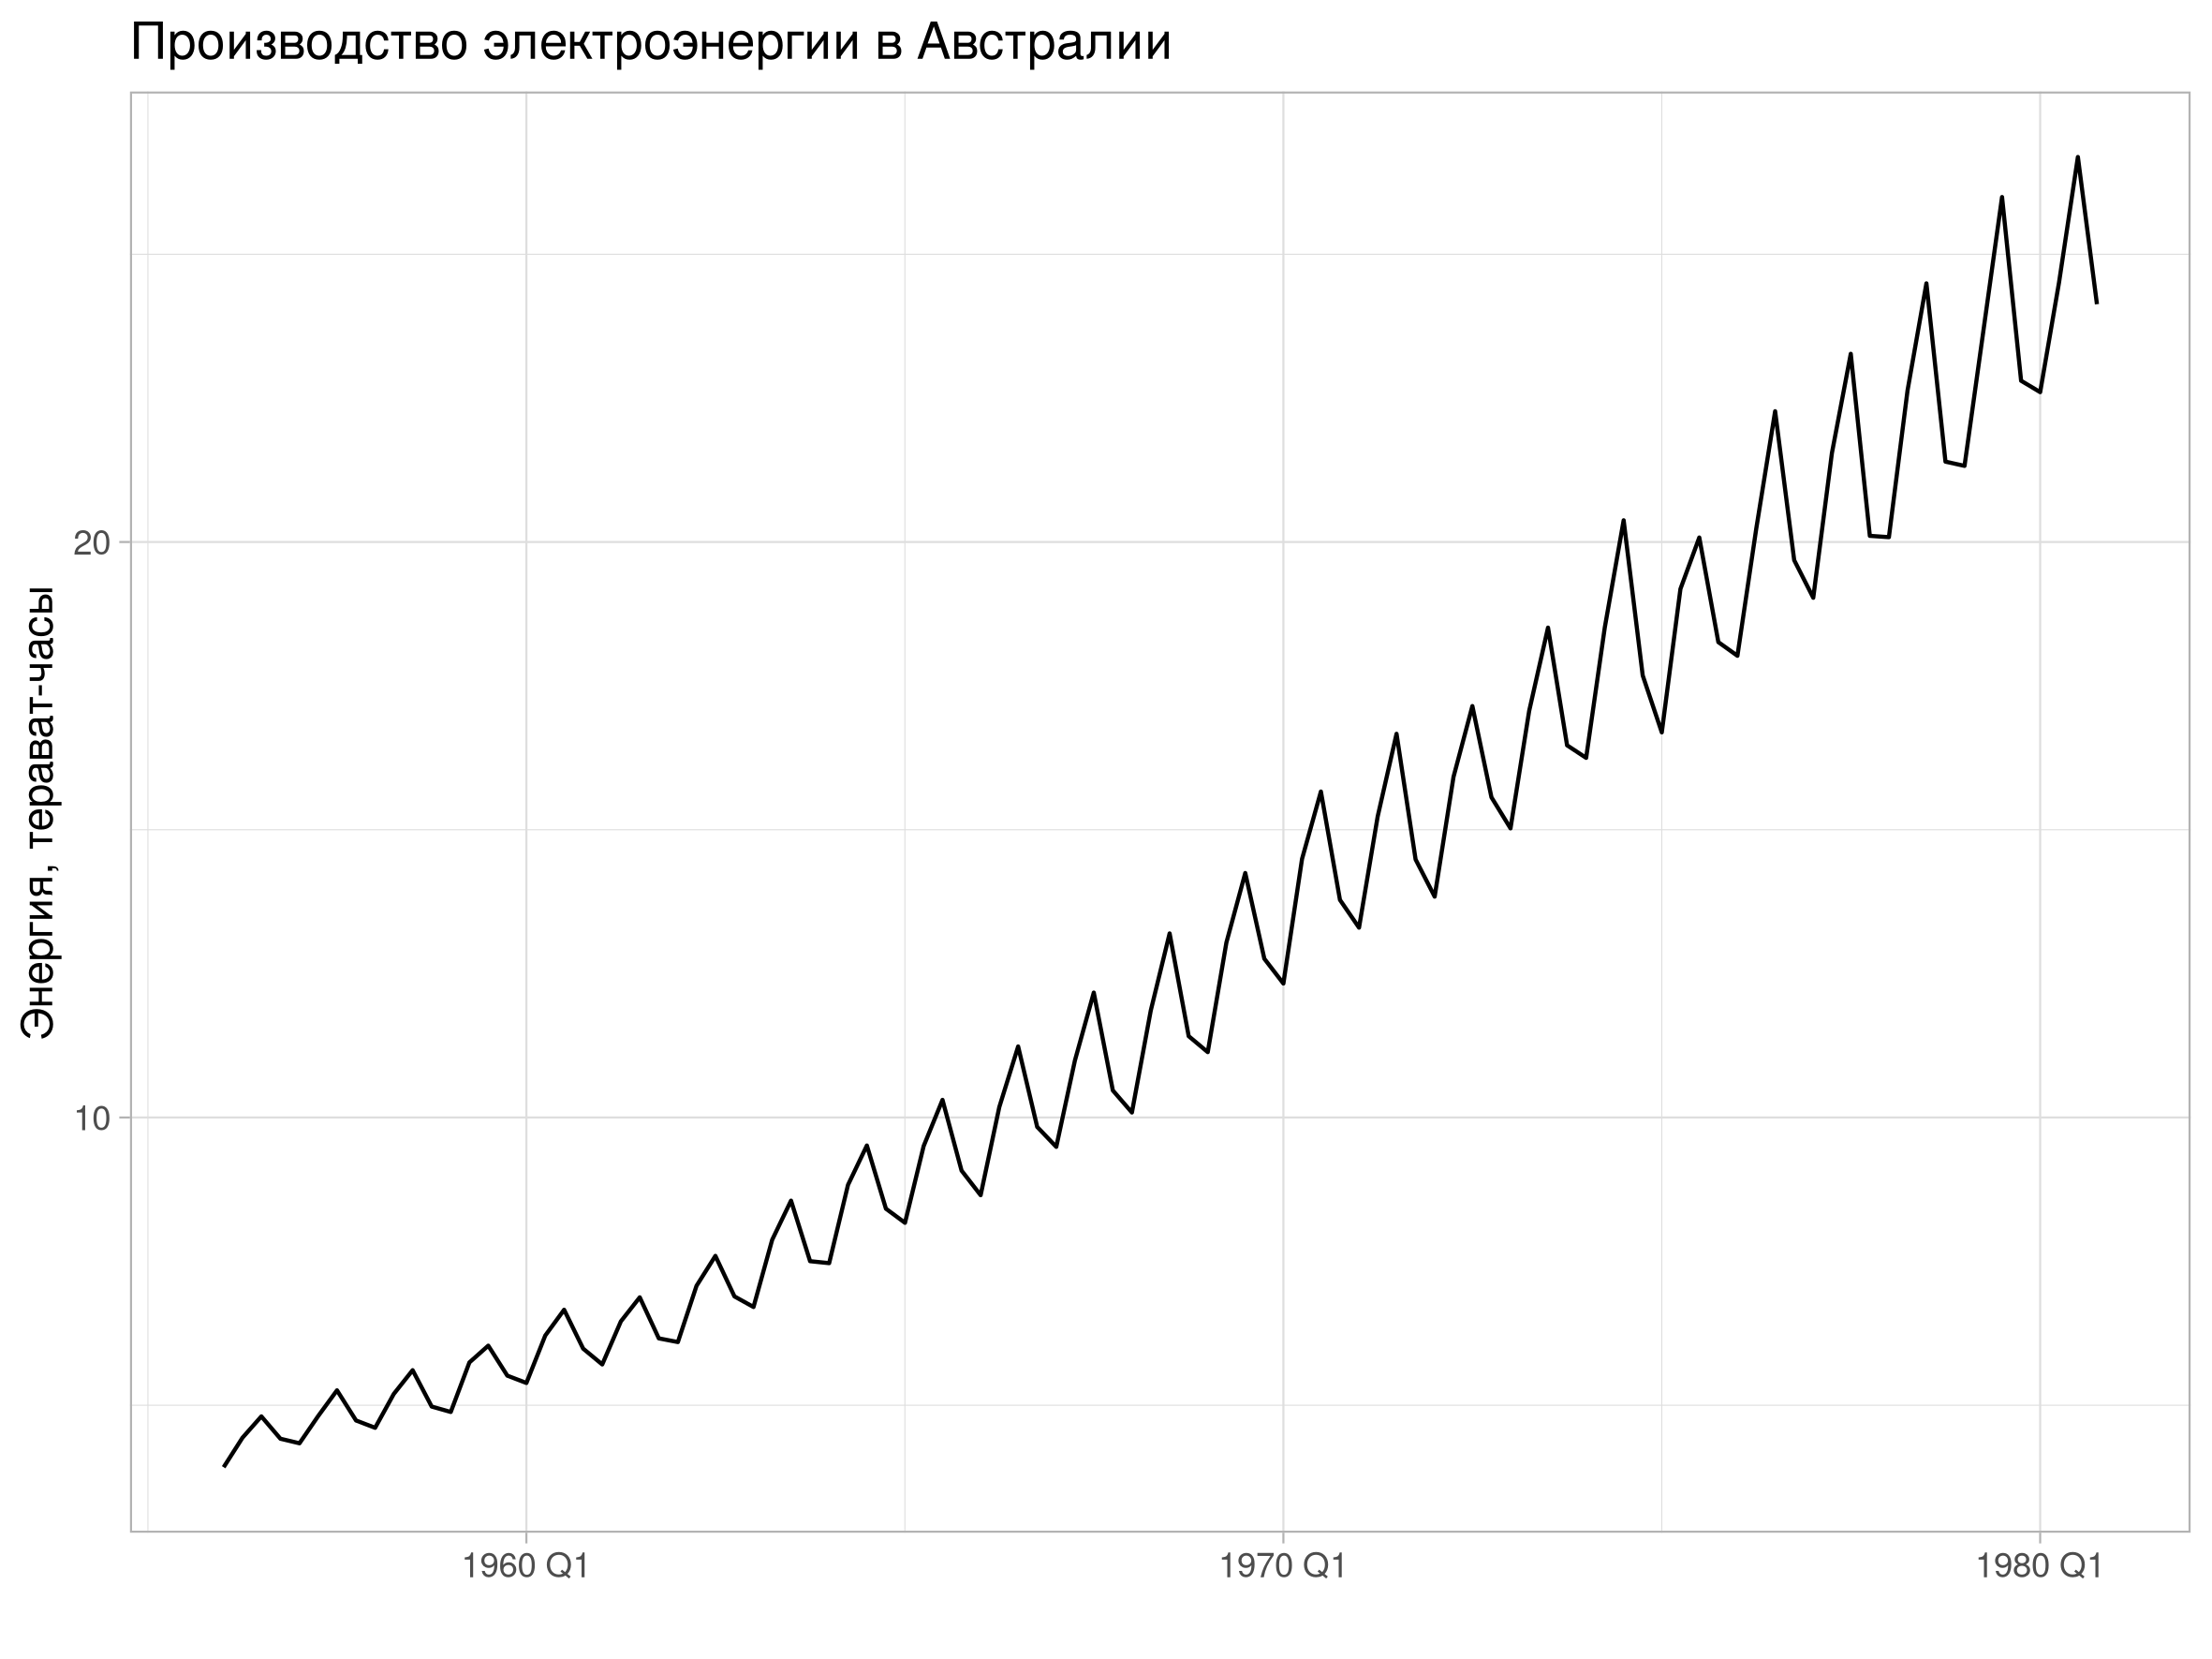
\includegraphics[width=\textwidth]{pictures/om_ts_03-033.png}

\end{frame}


\begin{frame}  
  \frametitle{Разная амплитуда колебаний}

  Возможные \alert{решения}:
  \begin{itemize}[<+->]
    \item Переход к логарифмам, $y_t \to \ln y_t$.
    \item Преобразование Бокса-Кокса, $y_t \to bc(y_t, \lambda)$.
    \item Мультипликативные компоненты. 
  \end{itemize}

\end{frame}



\begin{frame}
  \frametitle{ETS(MNM): уравнения}

  ETS(MNM) для месячных данных:
  
  \[
    \begin{cases}
     y_t = \ell_{t-1} \cdot s_{t-12} \cdot (1 + u_t); \\
    \ell_t = \ell_{t-1}\cdot  (1 + \alpha u_t), \text{ стартовое } \ell_0; \\
    s_t = s_{t-12}\cdot (1 + \gamma u_t), \text{ стартовые } s_0, \ldots, s_{-11}; \\
    u_t \sim \dN(0;\sigma^2) \text{ и независимы.} \\
    \end{cases}
  \]

  \pause
  ETS(ANA):
  \[
    \begin{cases}
     y_t = \ell_{t-1} + s_{t-12} + u_t; \\
    \ell_t = \ell_{t-1} + \alpha u_t, \text{ стартовое } \ell_0; \\
    s_t = s_{t-12} + \gamma u_t, \text{ стартовые } s_0, \ldots, s_{-11}; \\
    \end{cases}
  \]

\end{frame}



\begin{frame}
  \frametitle{ETS(MNM): параметры}

  ETS(MNM) для месячных данных:
  
  \[
    \begin{cases}
     y_t = \ell_{t-1} \cdot s_{t-12} \cdot (1 + u_t); \\
    \ell_t = \ell_{t-1}\cdot  (1 + \alpha u_t), \text{ стартовое } \ell_0; \\
    s_t = s_{t-12}\cdot (1 + \gamma u_t), \text{ стартовые } s_0, \ldots, s_{-11}; \\
    u_t \sim \dN(0;\sigma^2) \text{ и независимы.} \\
    \end{cases}
  \]

\pause
\alert{Несезонные} параметры: $\alpha$, $\sigma^2$, $\ell_0$.

\pause
\alert{Сезонные} параметры: $\gamma$, $s_0$, $s_{-1}$, \ldots, $s_{-11}$.

\pause
\alert{Ограничение}: $s_0 \cdot s_{-1} \cdot \ldots \cdot s_{-11} = 1$.

\pause
Всего: 15 параметров. 

\end{frame}

\begin{frame}
  \frametitle{Единицы измерения}

  Ряды $y_t$, $\ell_t$  — \alert{исходные} единицы измерения. 

  \pause

  Ряды $s_t$, $u_t$ — доли. 

  \pause

  Ряд $s_t$ измеряется относительно единицы, например, $s_t = 0.9$ — ниже тренда на 10\%.

  Ряд $u_t$ измеряется относительно нуля, например, $u_t = -0.1$ — падение на 10\%.

\end{frame}



\begin{frame}
  \frametitle{ETS(MNM): прогнозируем}

  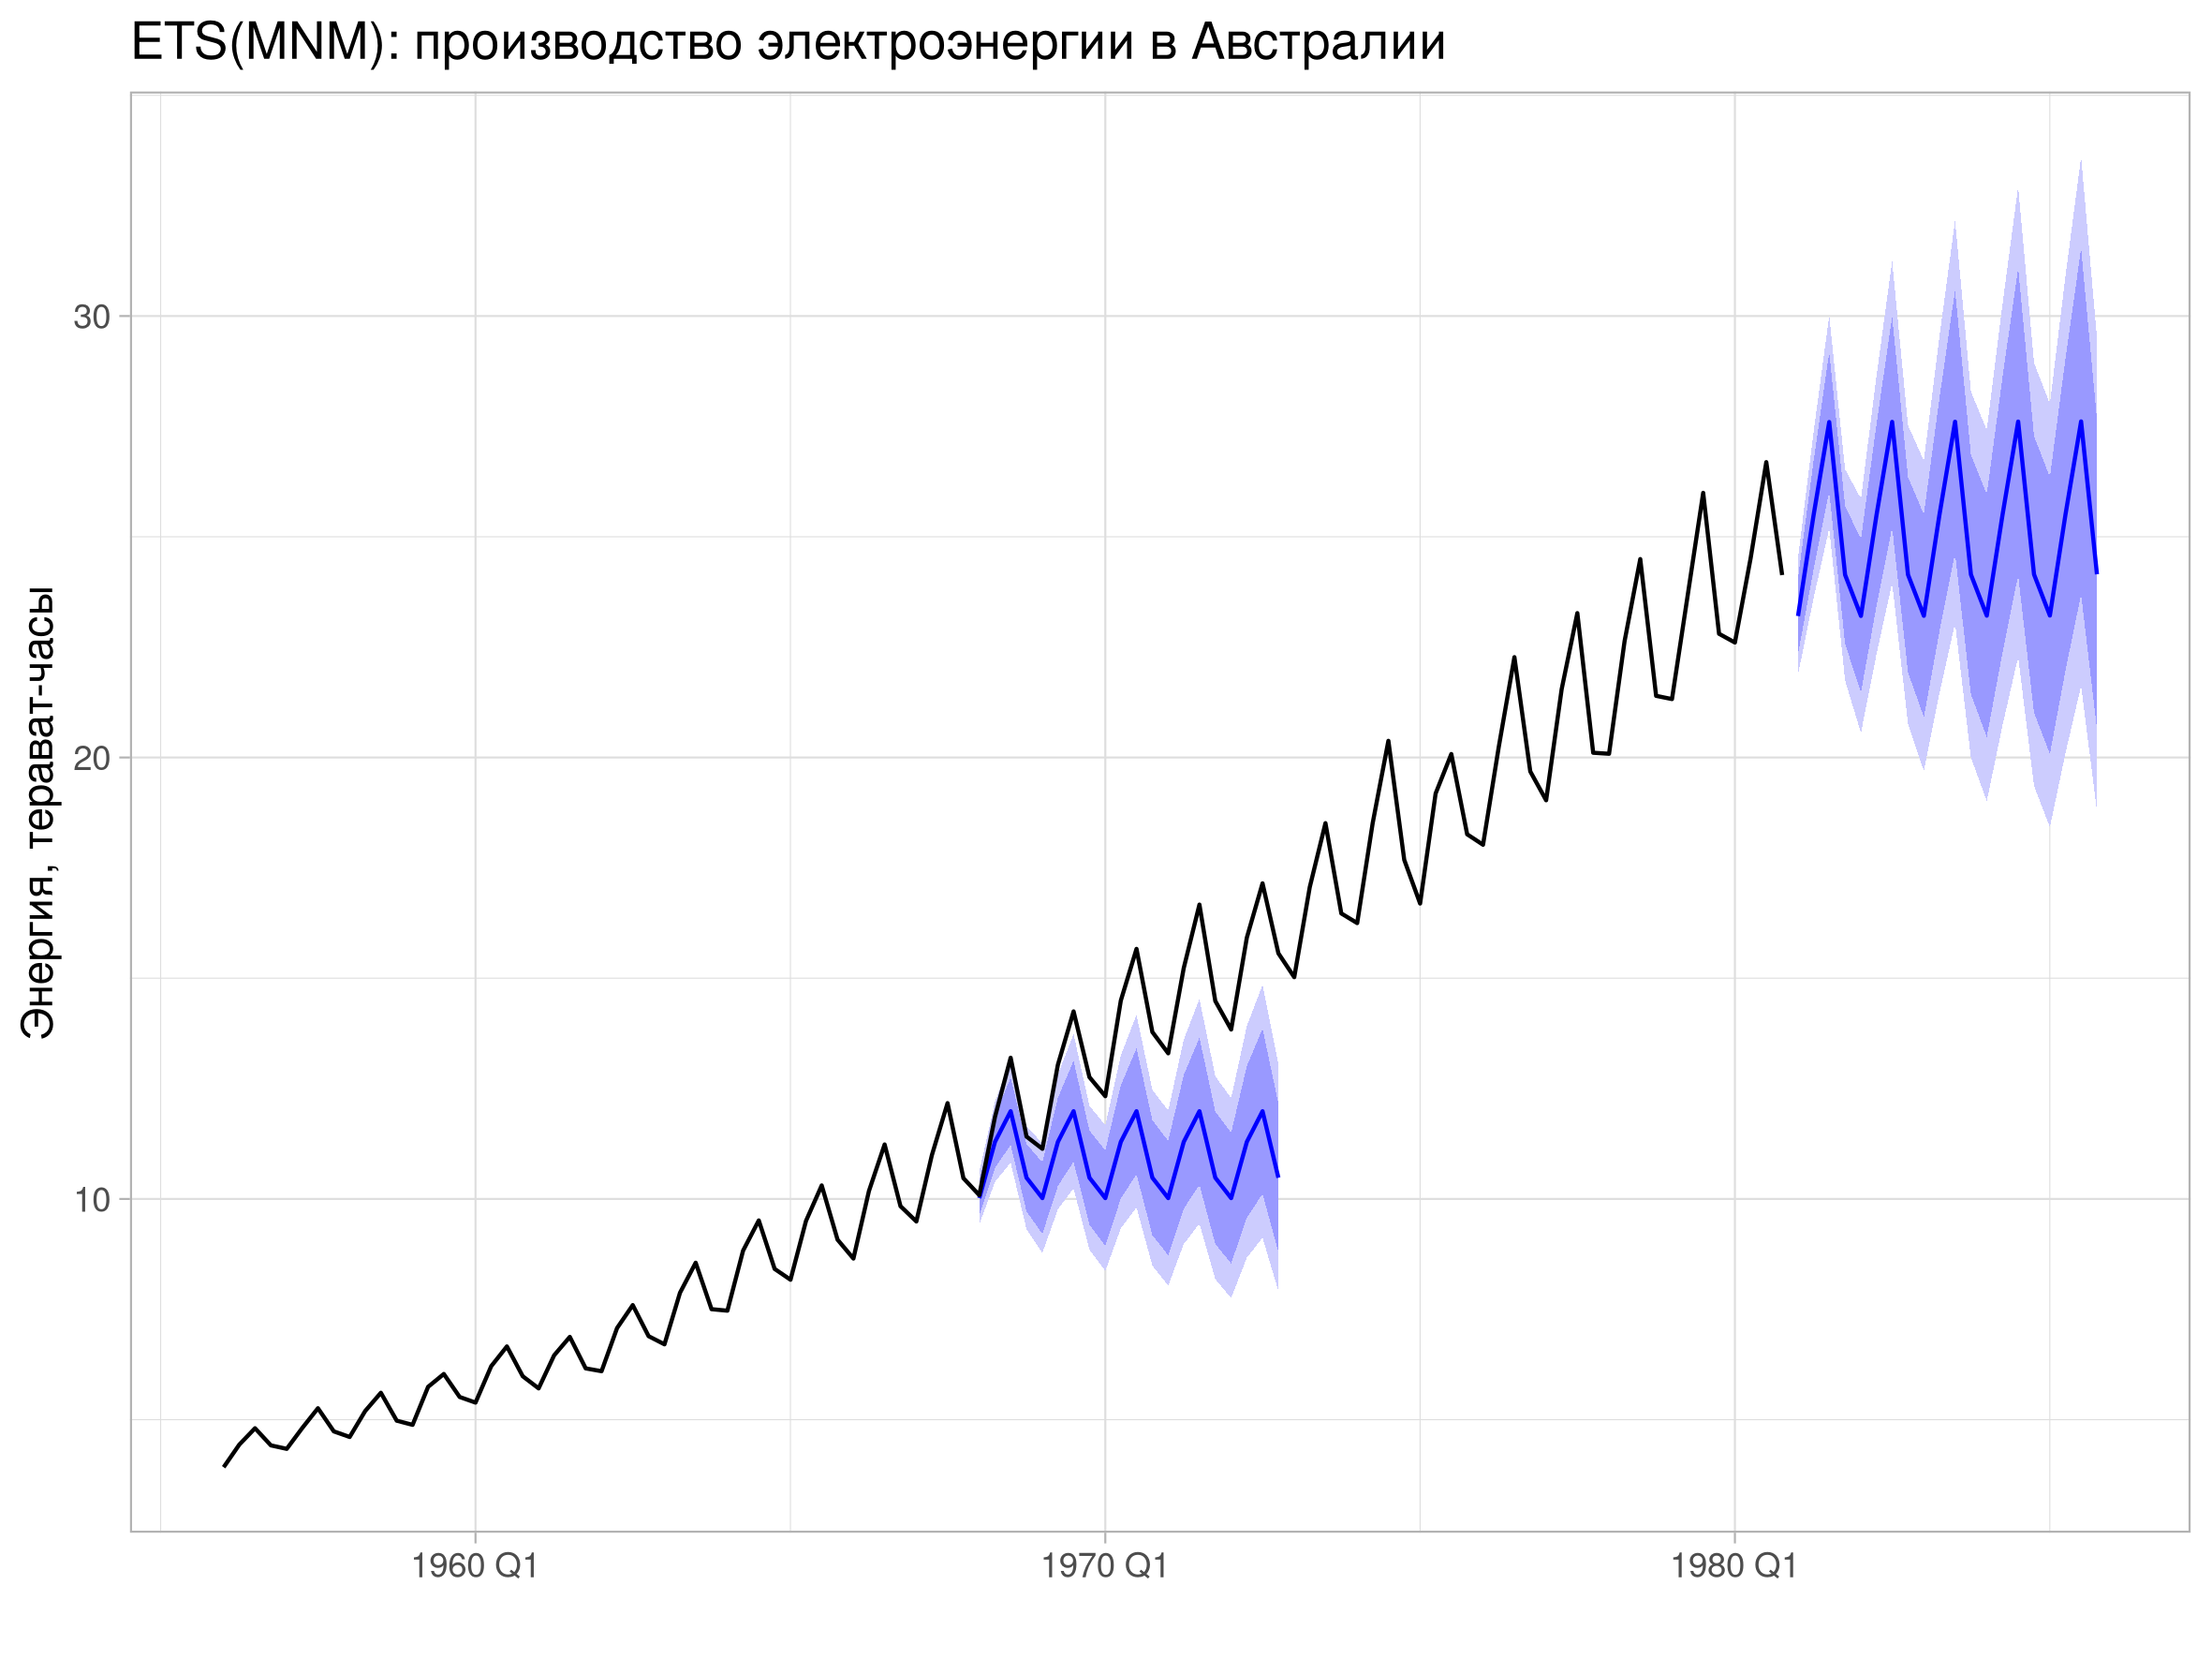
\includegraphics[width=\textwidth]{pictures/om_ts_03-047.png}


\end{frame}


\begin{frame}
  \frametitle{Прогноз на 1 шаг вперёд}

  \[
    \begin{cases}
     y_t = \ell_{t-1} \cdot s_{t-12} \cdot (1 + u_t); \\
    \ell_t = \ell_{t-1}\cdot  (1 + \alpha u_t), \text{ стартовое } \ell_0; \\
    s_t = s_{t-12}\cdot (1 + \gamma u_t), \text{ стартовые } s_0, \ldots, s_{-11}; \\
    u_t \sim \dN(0;\sigma^2) \text{ и независимы.} \\
    \end{cases}
  \]
  \pause
\[
y_{T+1} = \ell_T \cdot s_{T-11} \cdot (1 + u_{T+1})  
\]
\pause
\[
  (y_{T+1} \mid \mathcal F_T) \sim \dN(\ell_T \cdot s_{T-11} ; (\ell_T \cdot s_{T-11})^2\sigma^2)  
\]

\end{frame}


\begin{frame}
  \frametitle{Прогноз на 2 шага вперёд}

  \[
    \begin{cases}
     y_t = \ell_{t-1} \cdot s_{t-12} \cdot (1 + u_t); \\
    \ell_t = \ell_{t-1}\cdot  (1 + \alpha u_t), \text{ стартовое } \ell_0; \\
    s_t = s_{t-12}\cdot (1 + \gamma u_t), \text{ стартовые } s_0, \ldots, s_{-11}; \\
    u_t \sim \dN(0;\sigma^2) \text{ и независимы.} \\
    \end{cases}
  \]
  \pause
  \begin{multline*}
    y_{T+2} = \ell_{T+1} \cdot s_{T-10} \cdot(1 + u_{T+2}) = \\
    = \ell_T (1 + \alpha u_{T+1})\cdot s_{T-10} \cdot(1 + u_{T+2})
  \end{multline*}
   \pause
 \[
 (y_{T+2} \mid \mathcal F_T) \overset{\cdot}{\sim} \dN(\ell_T \cdot s_{T-10}; \ldots )
 \]
  
\end{frame}



\begin{frame}{Мультипликативная ETS: итоги}

  \begin{itemize}[<+->]
    \item Моделирует \alert{разную} амплитуду колебаний. 
    \item Для \alert{положительных рядов}.
    \item Простор для новых \alert{комбинаций}.
  \end{itemize}
\end{frame}



